\section{Aufbau}

Der Aufbau besteht aus einem dünnen, von der Decke hängenden Stahlseil, an dessen Ende eine Metallkugel befestigt ist. An der Wand hinter dem Pendel befindet sich eine Winkelskala. Die Messungen werden erneut mit Hilfe einer Lichtschranke duchgeführt.

\section{Bestimmung der Fallbeschleunigung}

\section{Mathematische Grundlagen}

Um die Fallbeschleunigung g der Erde mit Hilfe eines Pendels zu bestimmen, muss man zunächst eine Entscheidung darüber fällen, ob man mit dem Modell eines mathematischen oder eines physikalischen Pendels modellieren sollte.
In diesem Versuch wird das physikalische Pendel verwendet, da die Versuchbedinungen nicht idealisiert waren und das mathematische Modell daher zu ungenau wäre.

Da das Pendel für diesen Versuch um kleinen Winkel von ca. 5° augelenkt wurde, wird auf die Kleinwinkelannäherung des physikalischen Pendels zurückgegriffen

\begin{align}
	\label{eq:physikalisches-pendel}
	T = 2 \pi \sqrt{\frac{\theta}{m g d}}  \implies T^2 = 4 \pi^2 \frac{\theta}{m g d} \implies g = \frac{4 \pi^2 \theta}{m d T^2} .
\end{align}

Das Trägheitsmoment $\theta$ des Pendels setzt sich aus dem Trägheitsmoment der Kugel und dem Trägheitsmoment nach dem Satz von Steiner zusammen.
Da man die Kugel als Kugelkreisel ansehen kann, ergibt sich vereinfacht

\begin{align}
	\theta = \theta_\text{Kugel} + \theta_\text{Steiner} = \frac{2}{5} m r^2 + m d^2 .
\end{align}

Nach einsetzen in \ref{eq:physikalisches-pendel} ergibt sich

\begin{align}
	\label{eq:ortsfaktor}
	g = \frac{4 \pi^2 m (\frac{2}{5} r^2 + d^2)}{m d T^2} = 4 \pi^2 \frac{\frac{2}{5} r^2 + d^2}{d T^2}
\end{align} .

Die Periodendauer $T$ errechnet sich aus den Messwerten des Versuchs, die Länge $d$ des Pendelfadens ist als 2,355m gegeben und mit einem systematischen Fehler von 3mm behaftet.

Zuletzt wird der Radius der Kugel benötigt. Um diesen zu ermitteln, wurde der Durchmesser $D$ der Kugel dreimal mit einem Messschieber gemessen und über die Werte gemittelt.

\section{Durchführung und Auswertung}

Während dem Versuch wurde das Pendel 10 mal um einen kleinen Winkel von ca. 5° augelenkt und jeweils die Zeit gemessen, bis die vorgegebene Zahl an Perioden durchlaufen wurde.

\begin{table}[h!]
    \begin{center}
        \caption{Messwerte von Versuch 2.1}
        \begin{tabular}{cccc}
            \hline
            Perioden  & $T in s$  \\
            \hline
            1                   & 3,051		\\
            3                   & 9,206		\\
            5                   & 15,360	\\
            7                   & 21,515	\\
            9                   & 27,672	\\
            11                  & 33,828	\\
            13                  & 39,985	\\
            15                  & 46,145	\\
	        17                  & 52,300	\\
	        19                  & 58,471	\\
            \hline
            \label{tab:2_1-werte}
        \end{tabular}
    \end{center}
\end{table}


Die Berechnung der Periodendauer wird durch Regression ausgeführt.

\begin{figure}[h!]
    \centering
    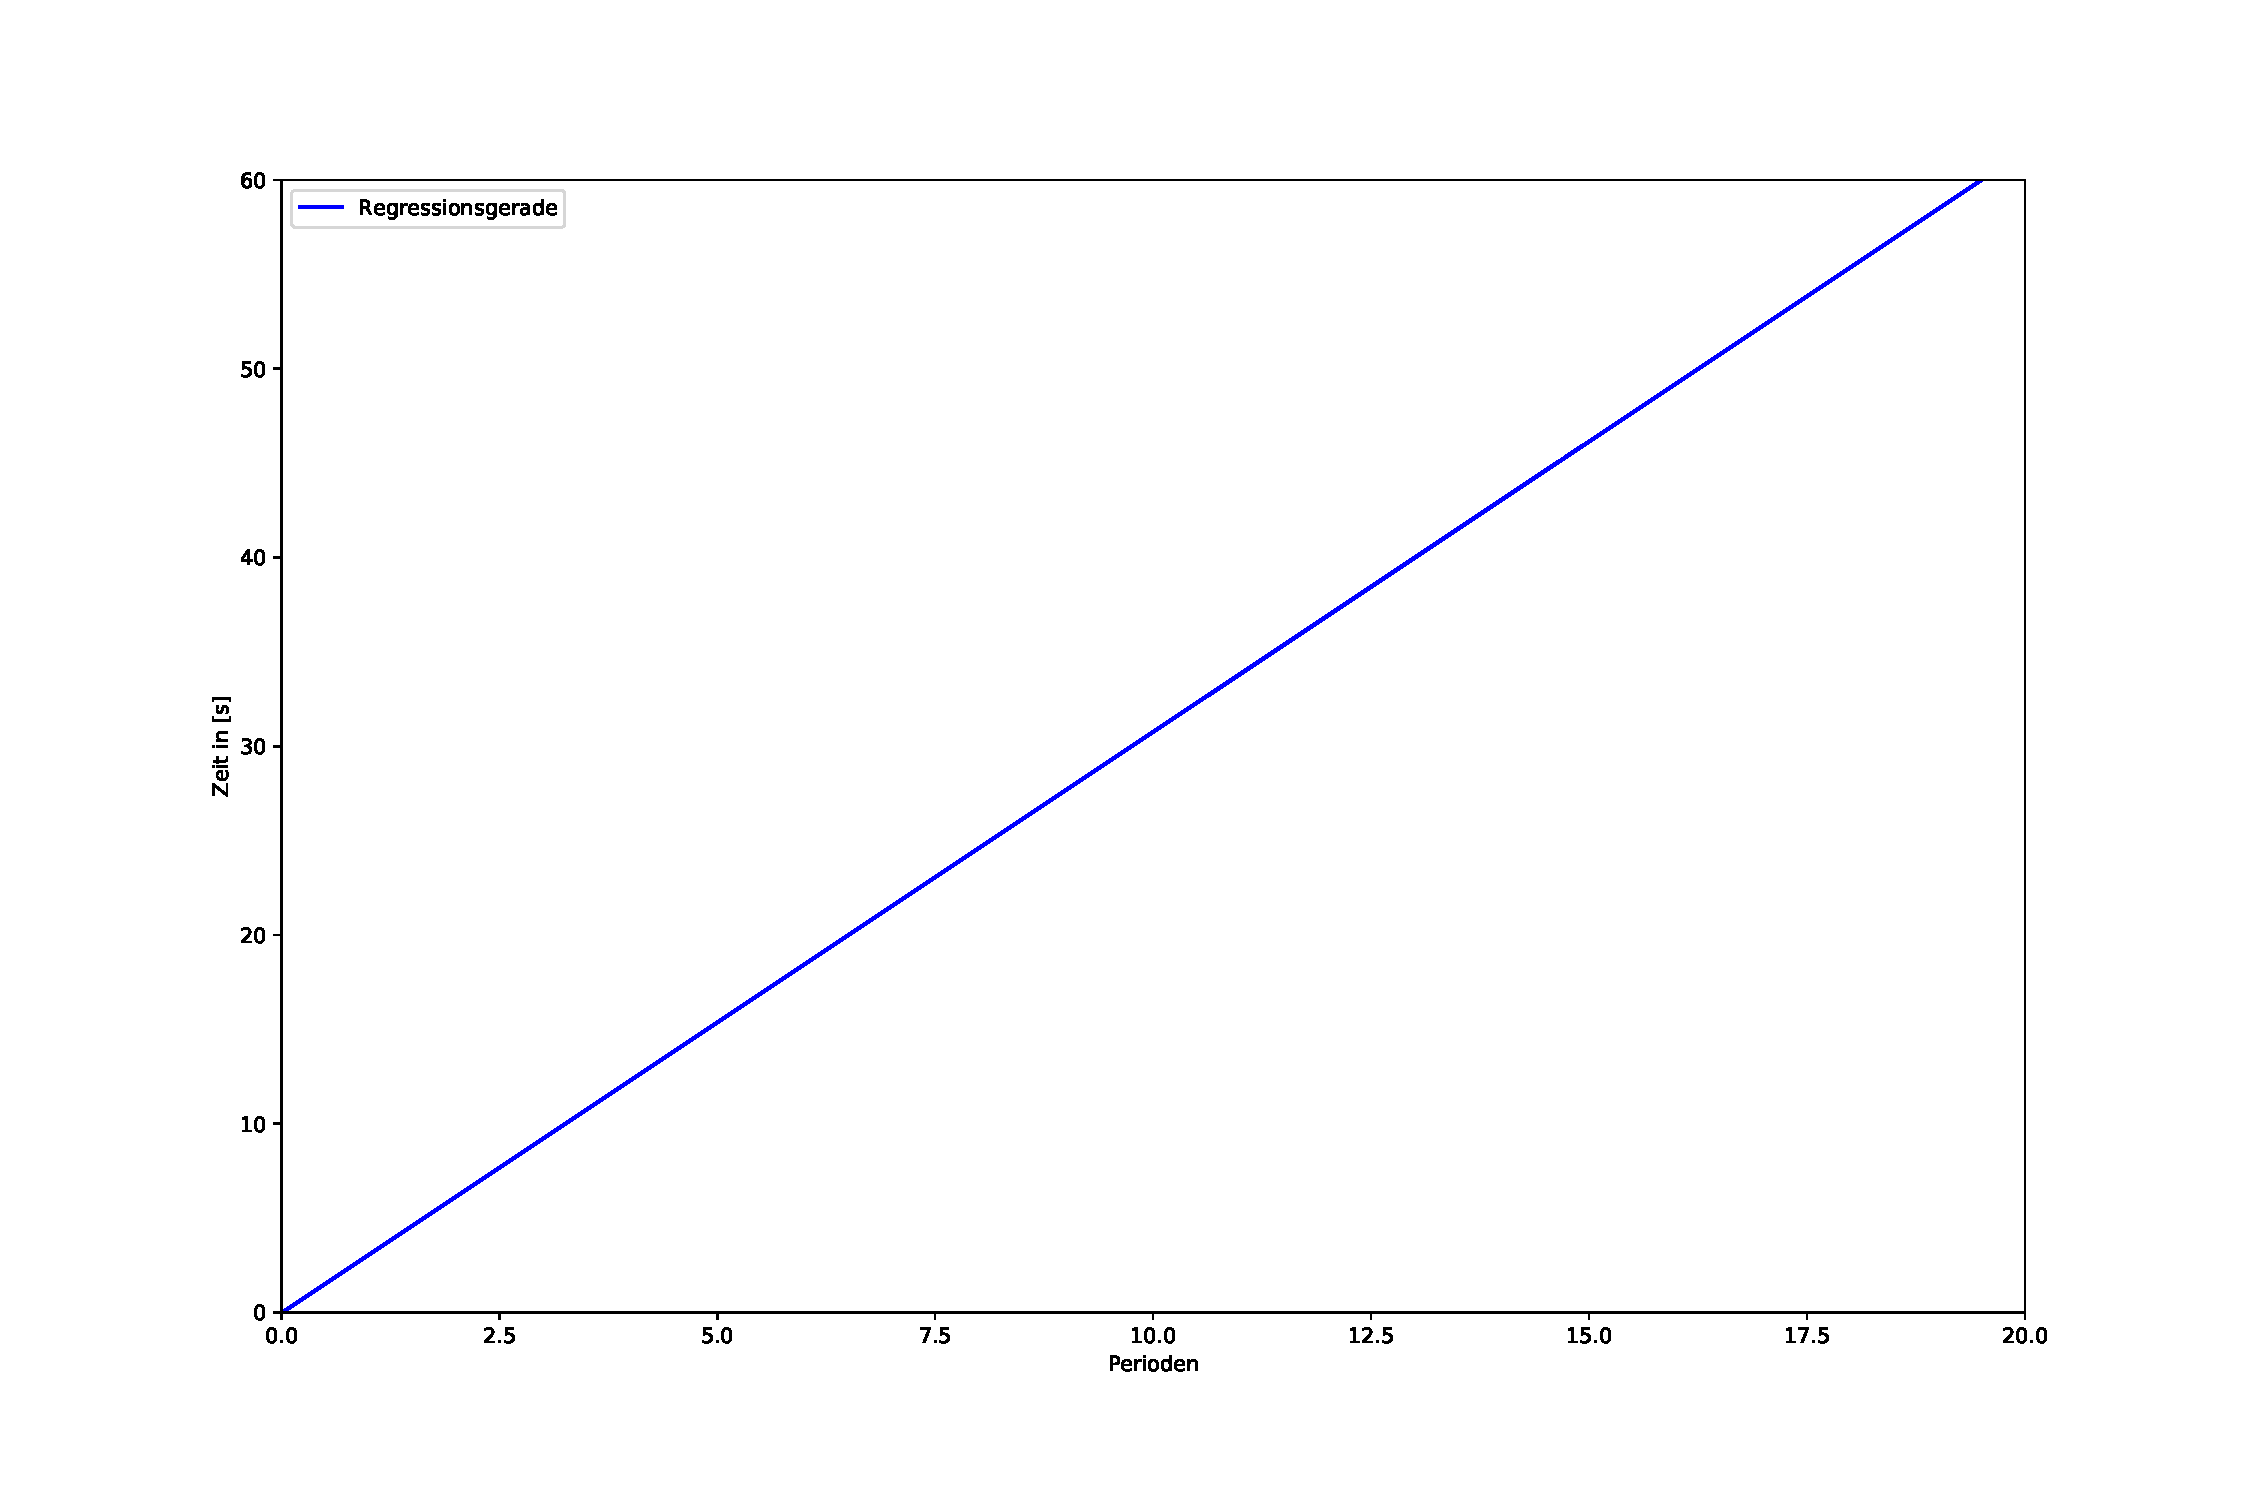
\includegraphics[scale=0.4]{./Pendel/Protokoll/fig/Fadenpendel_Regression.pdf}
    \caption{Plot der Messpunkte und der Regression}
    \label{fig:Faden_Reg1}
\end{figure}

Aus der Regression ergibt sich für $T$ ein Wert von $3.079s$, mit einer statistischen Fehlerbehaftung von $0,000018s$.

Der Radius der Kugel errechnet sich wie folgt:

$D_M = \frac{D_1 + D_2 + D_3}{3}$
$r = \frac{D_M}{2}$

Der Durchmesser der Kugel wurde zu $0,060m$, $0,059m$ und $0,060m$ gemessen.
Aufgrund der Ungenauigkeit des Messchiebers, werden die $D_i$ mit einem systematischen Fehler von $0,005m$ behaftet, wozu noch eine Standardabweichung zu $0,0006$m als statistischer Fehler hinzukommt.

Es ergibt sich demnach $r = 0,03m$ mit einem statistischen Fehler von $0,0003m$ und einem einem systematischen Fehler von $0,0025m$.

Nach \ref{eq:ortsfaktor} ergibt sich

$g = 9,8075\frac{m}{s^2}$

Zur Fehlerrechnung wird Gaußsche Fehlerfortpflanzung verwendet. Dies ist möglich, da man aufgrund der ungenauen Messmethode den Zusammenhang von r und d vernachlässigen kann und somit alle Fehler unkorreliert sind.

\section{Abhängigkeit der Schwingungsdauer von der Schwingungsweite}

Im zweiten Teil des Versuches wird die Beziehung zwischen der Schwingungsdauer und dem Auslenkungswinkel des Pendels untersucht.
Dazu wurde die Periodendauer jeweils für Winkel von 5° bis 60° in fünfer Schritten gemessen,
wobei für jede Messung 5 Perioden durchlaufen wurden.
Das Einstellen der Auslenkung des Pendels war durch die Natur des Versuchsaufbaus nicht genau möglich.
Um zumindest grobe Fehler zu vermeiden, wurde das Pendel von einer Person unter der Anleitung einer zweiten, weiter entfernten Person, ausgelenkt.

\section{Mathematische Grundlagen}

Die gemessenen Daten sollen mit einer Vorhersage verglichen werden.
Diesmal wird die Vorhersage mit dem Modell des mathematischen Pendels modelliert:

\begin{align}
	\ddot{\phi}(t) + \frac{g}{l} \cdot \sin ( \phi (t)) = 0
\end{align}

Analytisch ist diese Differenzialgleichung nicht lösbar, mit Hilfe der Taylorentwicklung kann man sie jedoch genügend annähern:

\begin{align}
	T(\phi) & = T_0 \sum_{n=0}^{\infty} \left( \frac{\left(2n\right)!}{\left(2^{n}n!\right)^2} \right)^2 \sin^{2n} \left(\phi /2\right) \\
& = T_0\cdot\left(1+\left(\frac{1}{2}\right)^2 \cdot \sin^2\left(\frac{\phi}{2}\right)+\left(\frac{1\cdot 3}{2\cdot 4}\right)^2 \cdot \sin^4\left(\frac{\phi}{2}\right) + \dots\right)
\end{align}

$T_0$ ist die Periodendauer für kleine Winkel, die aus dem ersten Versuchsteil übernommen werden kann.

\section{Auswertung}

\begin{table}[h!]
    \begin{center}
        \caption{Messwerte von Versuch 2.2}
        \begin{tabular}{cccc}
            \hline
            Auslenkwinkel in $ ^{\circ}$ & T in s \\
            \hline
            5                  & 15,357 \\
            10                & 15,380 \\
            15                & 15,409 \\
            20                & 15,463 \\
            25                & 15,524 \\
            30                & 15,609 \\
            35                & 15,709 \\
            40                & 15,820 \\
            45                & 15,950 \\
            50                & 16,057 \\
            55                & 16,257 \\
            60                & 16,423 \\
            \hline
            \label{tab:2_2-werte}
        \end{tabular}
    \end{center}
\end{table}


Die Messung und die Vorhersage werden nun zum visuellen Vergleich gemeinsam geplottet.

